\documentclass[12pt]{article}
\usepackage{../../format}
\lhead{A Level Physics}
\setcounter{secnumdepth}{5}
\usepackage[compat=1.1.0]{tikz-feynman}

%REMINDER: This needs to be compiled with LuaLaTeX to work

\begin{document}
\begin{center}
\underline{\huge Paper 1 Cheat Sheet}
\end{center}
\section{Measurements and their errors}
\textbf{Precision} - There is very little spread around the mean value\\
\textbf{Repeatability} - If the same experimenter repeats the investigation using the same method and equipment and obtains the same results\\
\textbf{Reproducibility} - If a different experimenter repeats the investigation, or uses a different experiment or technique, the same results are obtained\\
\textbf{Accuracy} - Close to the true value\\
{\renewcommand{\arraystretch}{2}
\begin{tabularx}{\textwidth}{|X|X|}
\hline
Combination&Operation\\
\hline
Adding or subtracting\newline $a=b+c$&Add the absolute uncertainties\newline $\Delta a=\Delta b+\Delta c$\\
\hline
Multiplying values\newline $a=b\times c$&Add the percentage uncertainties\newline $\epsilon a=\epsilon b+\epsilon c$\\
\hline
Dividing values\newline $a=\dfrac{b}{c}$&Add the percentage uncertainties\newline $\epsilon a=\epsilon b+\epsilon c$\\
\hline
Power rules\newline $a=b^c$&Multiply the percentage uncertainty by the power\newline $\epsilon a=c\times\epsilon b$\\
\hline
\end{tabularx}}
\newpage
\section{Particles and radiation}
\subsection{Constituents of the atom}
Protons and neurons in the centre, with shells of electrons around them
$$\textrm{Specific charge}=\frac{Q}{m}$$
\textbf{Isotope} - An atom with the same number of protons and electrons as an element, but a different number of neutrons
\subsection{Stable and unstable nuclei}
\subsubsection{The strong nuclear force}
\begin{tabular}{|c|c|}
\hline
$<0.5fm$&Repulsion\\
\hline
$0.5-3fm$&Attraction\\
\hline
$3fm+$&No force\\
\hline
\end{tabular}
\subsubsection{Alpha decay}
{\large
$$^A_ZX\rightarrow ^{A-4}_{Z-2}Y+^4_2\alpha$$
\subsubsection{Beta decay}
$$^A_ZX\rightarrow ^A_{Z+1}+^0_{-1}\beta+\overline{\nu}$$}
Neutrinos were hypothesised to allow for energy to be conserved in the interaction
\subsection{Particles, antiparticles and photons}
\subsubsection{Particle antiparticle pairs and their properties}
{\def\arraystretch{1.5}
\begin{tabularx}{\textwidth}{|X|X|X|}
\hline
\textbf{Property}&\textbf{Particle}&\textbf{Antiparticle}\\
\hline
Mass&x&x\\
\hline
\textcolor{red}{Charge}&x&-x\\
\hline
Rest Energy&x&x\\
\hline
\textcolor{red}{Baryon Number}&x&-x\\
\hline
\textcolor{red}{Lepton Number}&x&-x\\
\hline
\textcolor{red}{Strangeness}&x&-x\\
\hline
\end{tabularx}}
\newpage
\paragraph{Mesons}
\subparagraph{Pions(All 0 Strangeness)}
$ $\\
{\def\arraystretch{1.5}
\begin{tabularx}{\textwidth}{|X|X|}
\hline
$\pi^0$&$U\bar{U}$ or $D\bar{D}$\\
\hline
$\pi^+$&$U\bar{D}$\\
\hline
$\pi^-$&$D\bar{U}$\\
\hline
\end{tabularx}}
\subparagraph{Kaons (All strange)}
$ $\\
{\def\arraystretch{1.5}
\begin{tabularx}{\textwidth}{|X|X|}
\hline
$K^+$&$U\bar{S}$\\
\hline
$K^-$&$\bar{U}S$\\
\hline
$K^0$&$D\bar{S}$\\
\hline
$\bar{K^0}$&$\bar{D}S$\\
\hline
\end{tabularx}}
\subsubsection{The photon model of electromagnetic radiation}
A photon is a particle whose energy depends on its frequency. Formulas can be found on the data sheet to calculate this relationship
\subsubsection{Methods of annihilation and pair production}
\paragraph{Annihilation}
When a particle and an antiparticle meet, they annihilate each other, releasing two photons, with energy sum equivalent to the sum of the energy of the particle and antiparticle. This energy can be calculated from the rest energy values on the data sheet.
$$hf_{min}=E_0$$
\paragraph{Pair production}
In pair production a photon creates a particle and an antiparticle
$$hf_{min}=2E_0$$
\subsection{Particle interactions}
\subsubsection{The four fundamental interactions}
{\def\arraystretch{1.5}
\begin{tabularx}{\textwidth}{|X|X|X|X|}
\hline
\textbf{Force}&\textbf{Affects}&\textbf{Gauge Boson}&\textbf{Range}\\
\hline
Gravitational&Mass&Graviton&Infinite\\
\hline
Electromagnetic&Charge&Photon&Infinite\\
\hline
Nuclear Strong&Quarks&Gluon(Pion)&$10^{-15}$m\\
\hline
Nuclear Weak&Leptons+Quarks&$W^+,W^-,Z^0$&$10^{-18}$m\\
\hline
\end{tabularx}}
\newpage
\subsubsection{Diagrams to represent the interactions}
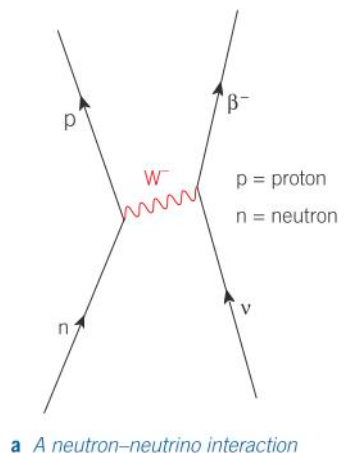
\includegraphics[width=6cm]{neutron-neutrino.png}
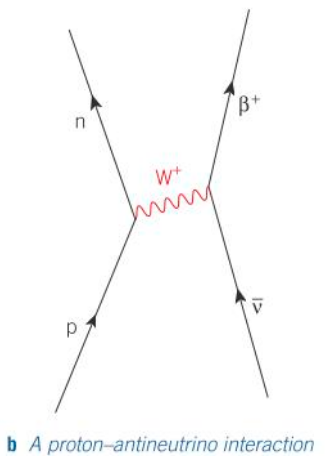
\includegraphics[width=6cm]{proton-antineutrino.png}
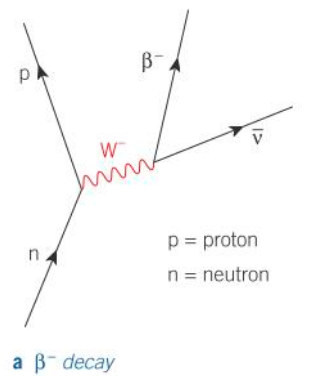
\includegraphics[width=6cm]{betaminus.png}
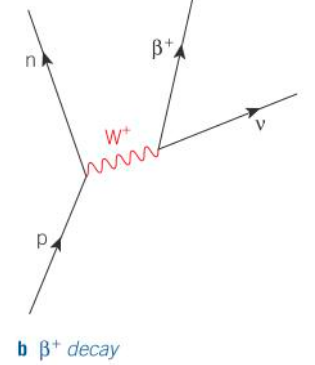
\includegraphics[width=6cm]{betaplus.png}
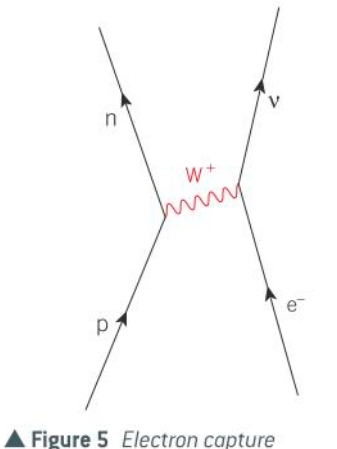
\includegraphics[width=6cm]{electron_capture.png}
\subsection{Classifications of particles}
{\renewcommand{\arraystretch}{2}
\begin{tabularx}{\textwidth}{|X|X|X|X|X|X|X|}
\hline
&\multicolumn{2}{|c|}{\centering Hadron}&\multicolumn{4}{|c|}{\centering Lepton}\\
\cline{2-7}
&Baryon&Meson&Electron&Muon&Electron neutrino&Muon neutrino\\
\hline
What it is&3 quarks&Quark antiquark pair&&&&\\
\hline
\end{tabularx}}
\paragraph{Baryons}
\begin{itemize}
\item Baryon number is conserved during interactions
\item The proton is the only stable baryon, all other baryons decay to it
\end{itemize}
\end{document}